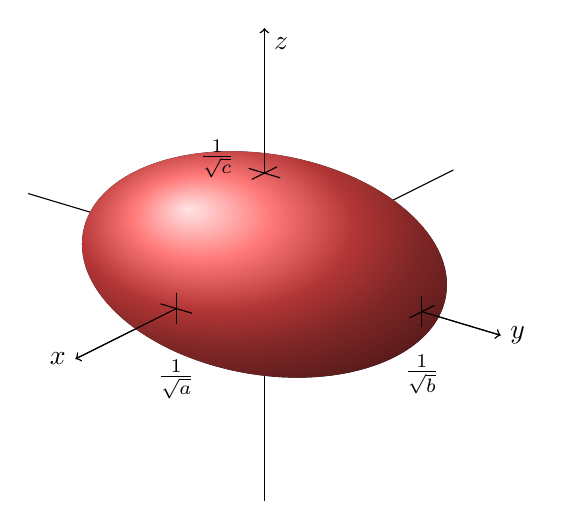
\begin{tikzpicture}[scale=2]
    \begin{scope}[y={(1cm,-0.3cm)},x={(-0.8cm,-0.4cm)},z={(0cm,1cm)}]
      \draw[->] (-1.5,0,0) -- (1.5,0,0) node[left] {$x$};
      \draw[->] (0,-1.5,0) -- (0,1.5,0) node[right] {$y$};
      \draw[->] (0,0,-1.5) -- (0,0,1.5) node[below right] {$z$};
    \end{scope}
    \fill[ball color=red!70] (0,0,0) circle [x radius=1.17, y radius=0.7, rotate=-10];
    \begin{scope}[y={(1cm,-0.3cm)},x={(-0.8cm,-0.4cm)},z={(0cm,1cm)}]
      \draw[->] (0.7,0,0) -- (1.5,0,0);
      \draw[->] (0,1,0) -- (0,1.5,0);
      \draw[->] (0,0,0.58) -- (0,0,1.5);
      \draw (0.7,0,0) -- +(0,0,0.1) -- +(0,0,-0.1) +(0,0,-0.45) node {$\frac{1}{\sqrt{a}}$};
      \draw (0.7,0,0) -- +(0,0.1,0) -- +(0,-0.1,0);
      \draw (0,1,0) -- +(0,0,0.1) -- +(0,0,-0.1) +(0,0,-0.4) node {$\frac{1}{\sqrt{b}}$};
      \draw (0,1,0) -- +(0.1,0,0) -- +(-0.1,0,0);
      \draw (0,0,0.58) -- +(-0.1,0,0) -- +(0.1,0,0);
      \draw (0,0,0.58) -- +(0,0.1,0) -- +(0,-0.1,0) +(0,-0.3,0) node {$\frac{1}{\sqrt{c}}$};
    \end{scope}
  \end{tikzpicture}
